\documentclass[conference]{IEEEtran}
\usepackage[utf8]{inputenc}
\usepackage{amsmath,amssymb,graphicx,booktabs}

\begin{document}

\title{Language JEPA for Reasoning: Predicting Answer Embeddings from Questions and Paraphrase Pairs}

\author{\IEEEauthorblockN{Dheiver Francisco Santos, PhD}
\IEEEauthorblockA{Independent Researcher\\
Maceió, Alagoas, Brazil\\
ORCID: https://orcid.org/0000-0002-8599-9436}}

\maketitle

\begin{abstract}
Autoregressive language models are trained to predict tokens, which couples the objective to surface form. We study a language joint-embedding predictive architecture that predicts the embedding of an answer from the embedding of a question, and that uses paraphrase pairs as an additional signal. We compare it with an autoregressive objective on arithmetic and multi-step reasoning tasks, and on a synthetic arithmetic setting where the correct answer is known by construction. A symbolic pilot shows that a small MLP readout fails beyond depth 2; the language JEPA results are pending.
\end{abstract}

\begin{IEEEkeywords}
language models, JEPA, reasoning, paraphrase, embedding prediction
\end{IEEEkeywords}

\section{Introduction}
Reasoning tasks reward the same answer under many surface forms. An objective that predicts answer embeddings rather than tokens may encourage representations invariant to paraphrase, but it may also lose the precision needed to produce an exact answer. We ask whether a language JEPA improves multi-step reasoning under matched compute, and whether paraphrase supervision is the cause of any gain.

\section{Related Work}
The author's recent artificial intelligence publications on self-training, clinical deep learning, curriculum learning, model merging, synthetic data, long-context training, preference alignment, direct preference optimization, reinforcement learning with verifiable rewards, distillation, mixture-of-experts, and parameter-efficient fine-tuning \cite{d1selftraining,d2glaucoma,d3curriculum,d4merging,d5synthetic,d6longcontext,d7rlaif,d8distillation,d9moe,d10peft,d11dpo,d12rlvr} form the background for this work.

JEPA-style prediction in embedding space is introduced for images and video \cite{bardes2024vjepa}. Its use for language is less studied. The author's recent work on Mixture-of-Experts training \cite{d9moe}, long-context training \cite{d6longcontext}, and parameter-efficient fine-tuning \cite{d10peft} provides the training setting used here. Preference-based alignment methods \cite{d7rlaif} are relevant as an alternative route to behavior control.

\section{Method}
Given a question $q$ and an answer $a$, an encoder $f_\theta$ produces $z_q = f_\theta(q)$ and a target encoder $\bar{f}$ produces $z_a = \bar{f}(a)$. The predictor $g_\phi$ is trained so that $g_\phi(z_q) \approx z_a$. Paraphrase pairs $(q, q')$ add a term that asks $g_\phi(f_\theta(q))$ and $g_\phi(f_\theta(q'))$ to agree. Decoding for an exact answer uses a small readout head trained on frozen predictions.

\subsection*{Equations and their meaning}
The synthetic task has operators $o_i\in\{-1,+1\}$ and values $v_i\in\{0,\dots,9\}$ for $i=1,\dots,k$. The answer is
\begin{equation}
y=\Big(\sum_{i=1}^{k}o_i\,v_i\Big)\bmod 10,
\end{equation}
so reasoning depth $k$ is the number of steps that must be combined.

The autoregressive baseline minimizes the negative log-likelihood of the answer tokens $a_t$ given the question $q$ and previous tokens:
\begin{equation}
\mathcal{L}_{\mathrm{AR}}=-\sum_{t}\log p_\theta\big(a_t\mid q,a_{<t}\big).
\end{equation}
The language JEPA predicts the answer embedding from the question embedding:
\begin{equation}
\mathcal{L}_{\mathrm{JEPA}}=\big\lVert g_\phi(f_\theta(q))-\bar f(a)\big\rVert_2^2,
\end{equation}
where $f_\theta$ encodes the question, $\bar f$ is the stop-gradient target encoder for the answer, and $g_\phi$ is the predictor. Paraphrase pairs $(q,q')$ add an agreement term $\lVert g_\phi(f_\theta(q))-g_\phi(f_\theta(q')) \rVert_2^2$, which asks paraphrases to map to the same prediction.

The readout accuracy over $N$ test items is
\begin{equation}
\mathrm{Acc}=\frac{1}{N}\sum_{n=1}^{N}\mathbf{1}\big[\hat y_n=y_n\big],
\end{equation}
where $\mathbf{1}[\cdot]$ is 1 when the predicted answer $\hat y_n$ equals the true answer $y_n$ and 0 otherwise. Chance level for ten classes is $0.1$.

\section{Experimental Protocol}
\textbf{Synthetic arithmetic.} Multi-step integer problems with a known solution, with depth $k \in \{1,2,3,4\}$, to measure accuracy as a function of reasoning depth.

\textbf{Benchmarks.} GSM8K-style word problems in English and Portuguese translations, with exact-match accuracy.

\textbf{Baselines.} Autoregressive fine-tuning with the same backbone and token budget; the same model without paraphrase pairs.

\textbf{Compute.} Matched number of training tokens and parameters. Compute is reported in FLOPs.

\textbf{Statistics.} Five seeds, 95\% bootstrap intervals, paired tests.

\section{Results}
This pilot arm uses symbolic arithmetic with a small MLP readout, not a language JEPA. Accuracy is 1.00 at depth $k=1$, 0.51 at $k=2$, and at chance level (about 0.10) for $k\geq 3$. The readout fails beyond shallow depth, so this arm gives no evidence about reasoning. The autoregressive baseline, the paraphrase ablation, and the language benchmarks remain pending.

\begin{figure}[!t]
\centering
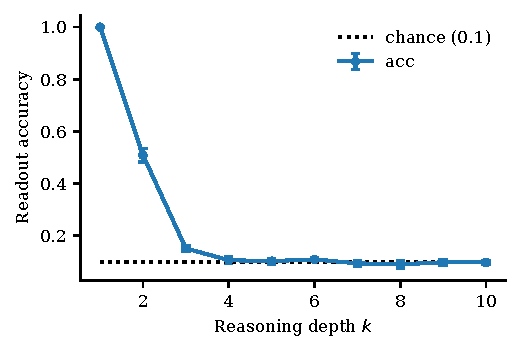
\includegraphics[width=\columnwidth]{figs/fig04_reasoning.pdf}
\caption{Readout accuracy versus reasoning depth on synthetic arithmetic (pilot, MLP). Dotted line: chance level.}
\label{fig:fig04_reasoning}
\end{figure}

\section{Discussion and Limitations}
The readout head adds a decoding step that could account for part of the difference, so the protocol reports results with and without it. Translation may change difficulty, so Portuguese and English are reported separately.

\section{Conclusion}
We propose a matched-compute comparison of answer-embedding prediction and autoregressive training on reasoning, with paraphrase supervision as an explicit ablation.

\section*{Acknowledgments}
The author thanks the Brazilian artificial intelligence community.

\nocite{ctl_full_names}
\bibliographystyle{IEEEtran}
\bibliography{refs}

\end{document}
